\documentclass{article}
\usepackage{amsmath}    % For mathematical symbols
\usepackage{booktabs}   % For professional table formatting
\usepackage{tabularx}   % For flexible tables
\usepackage{xcolor}     % For row colors
\usepackage{array}      % For flexible column formatting
\usepackage{graphicx}   % For including logos or images
\usepackage[a4paper, top=1in, bottom=1in, left=0.8in, right=0.8in]{geometry}
\usepackage{lipsum}   % For placeholder text
\usepackage{caption}
\usepackage{subcaption}

\setlength{\parskip}{1em}  % Adds 1em of vertical space between paragraphs

\begin{document}

% Title
\title{Foundations and Frontiers of Machine Learning\\Group Assignment 2\\Group 1}
\author{}
\date{}
\maketitle

% Table of Contents
\tableofcontents
\newpage

% Lists
\listoffigures
\listoftables
\newpage

% Sections
\section{Table of Contributions}

\begin{table}[h!]
    \centering
    \begin{tabular}{|l|l|l|}
        \hline
        \textbf{Name} & \textbf{Student ID} & \textbf{Contribution} \\ \hline
        Emmanouil Tsolias       & 239490757 & Graded Assignment 2 \\ \hline
    \end{tabular}
    \caption{Individual Contribution to Group Work}
    \label{tab:contributions}
\end{table}
\newpage

\section{Data Visualisation (Task 2)}
\subsection{Visualing with PCA}

Machine learning models use data to finetune the values of their internal parameters in a process called training.
The power of the classification model is closely related to the amount of relevant information contained in the dataset, thus bigger datasets are usually preferred.
However, not all information within the dataset is useful.
Oftentimes, a feature contains information that has already been made available by another feature or a combination thereof, and as number of features within a dataset grows larger, the chances that a feature consists of the linear combination of other features of the dataset increase.
At the same time, the mediums of visualising these datasets are usually books or electronic devices that are best suited for up to two features, as they physically have two dimensions.
Using techniques such as video or colour/shape encoding can increase that by some amount, but datasets can have dimensions in the order of millions, orders of magnitude higher than what humans can visualise or comprehend (Sarkar, 2018).

The issue of repeated information within the dataset can be addressed by constructing new features that encompass the dataset’s information without repetition, using with the Principal Components Analysis (PCA) technique.
The first new feature is engineered to explain as much variance as possible from all features of the dataset (Maćkiewicz, 1993).
Each next one is engineered to contain as much of the information that is left, without incorporating any information of the previously engineered features.
This often means that the last features contain little to no additional information (depending on how linearly independent the dataset was) and can be discarded, allowing for easier visualization and reducing the overall noise.
What is more, the features are now in descending order in terms of variance explained so we can select the first n ones, knowing that we have retain maximum information per feature.
We can now select a number that is suitable for visualization.
The new features have no actual meaning but can be used to show the distribution of the samples in the space, informing us about the separability of the classes.

\begin{figure}[h!]
    \centering
    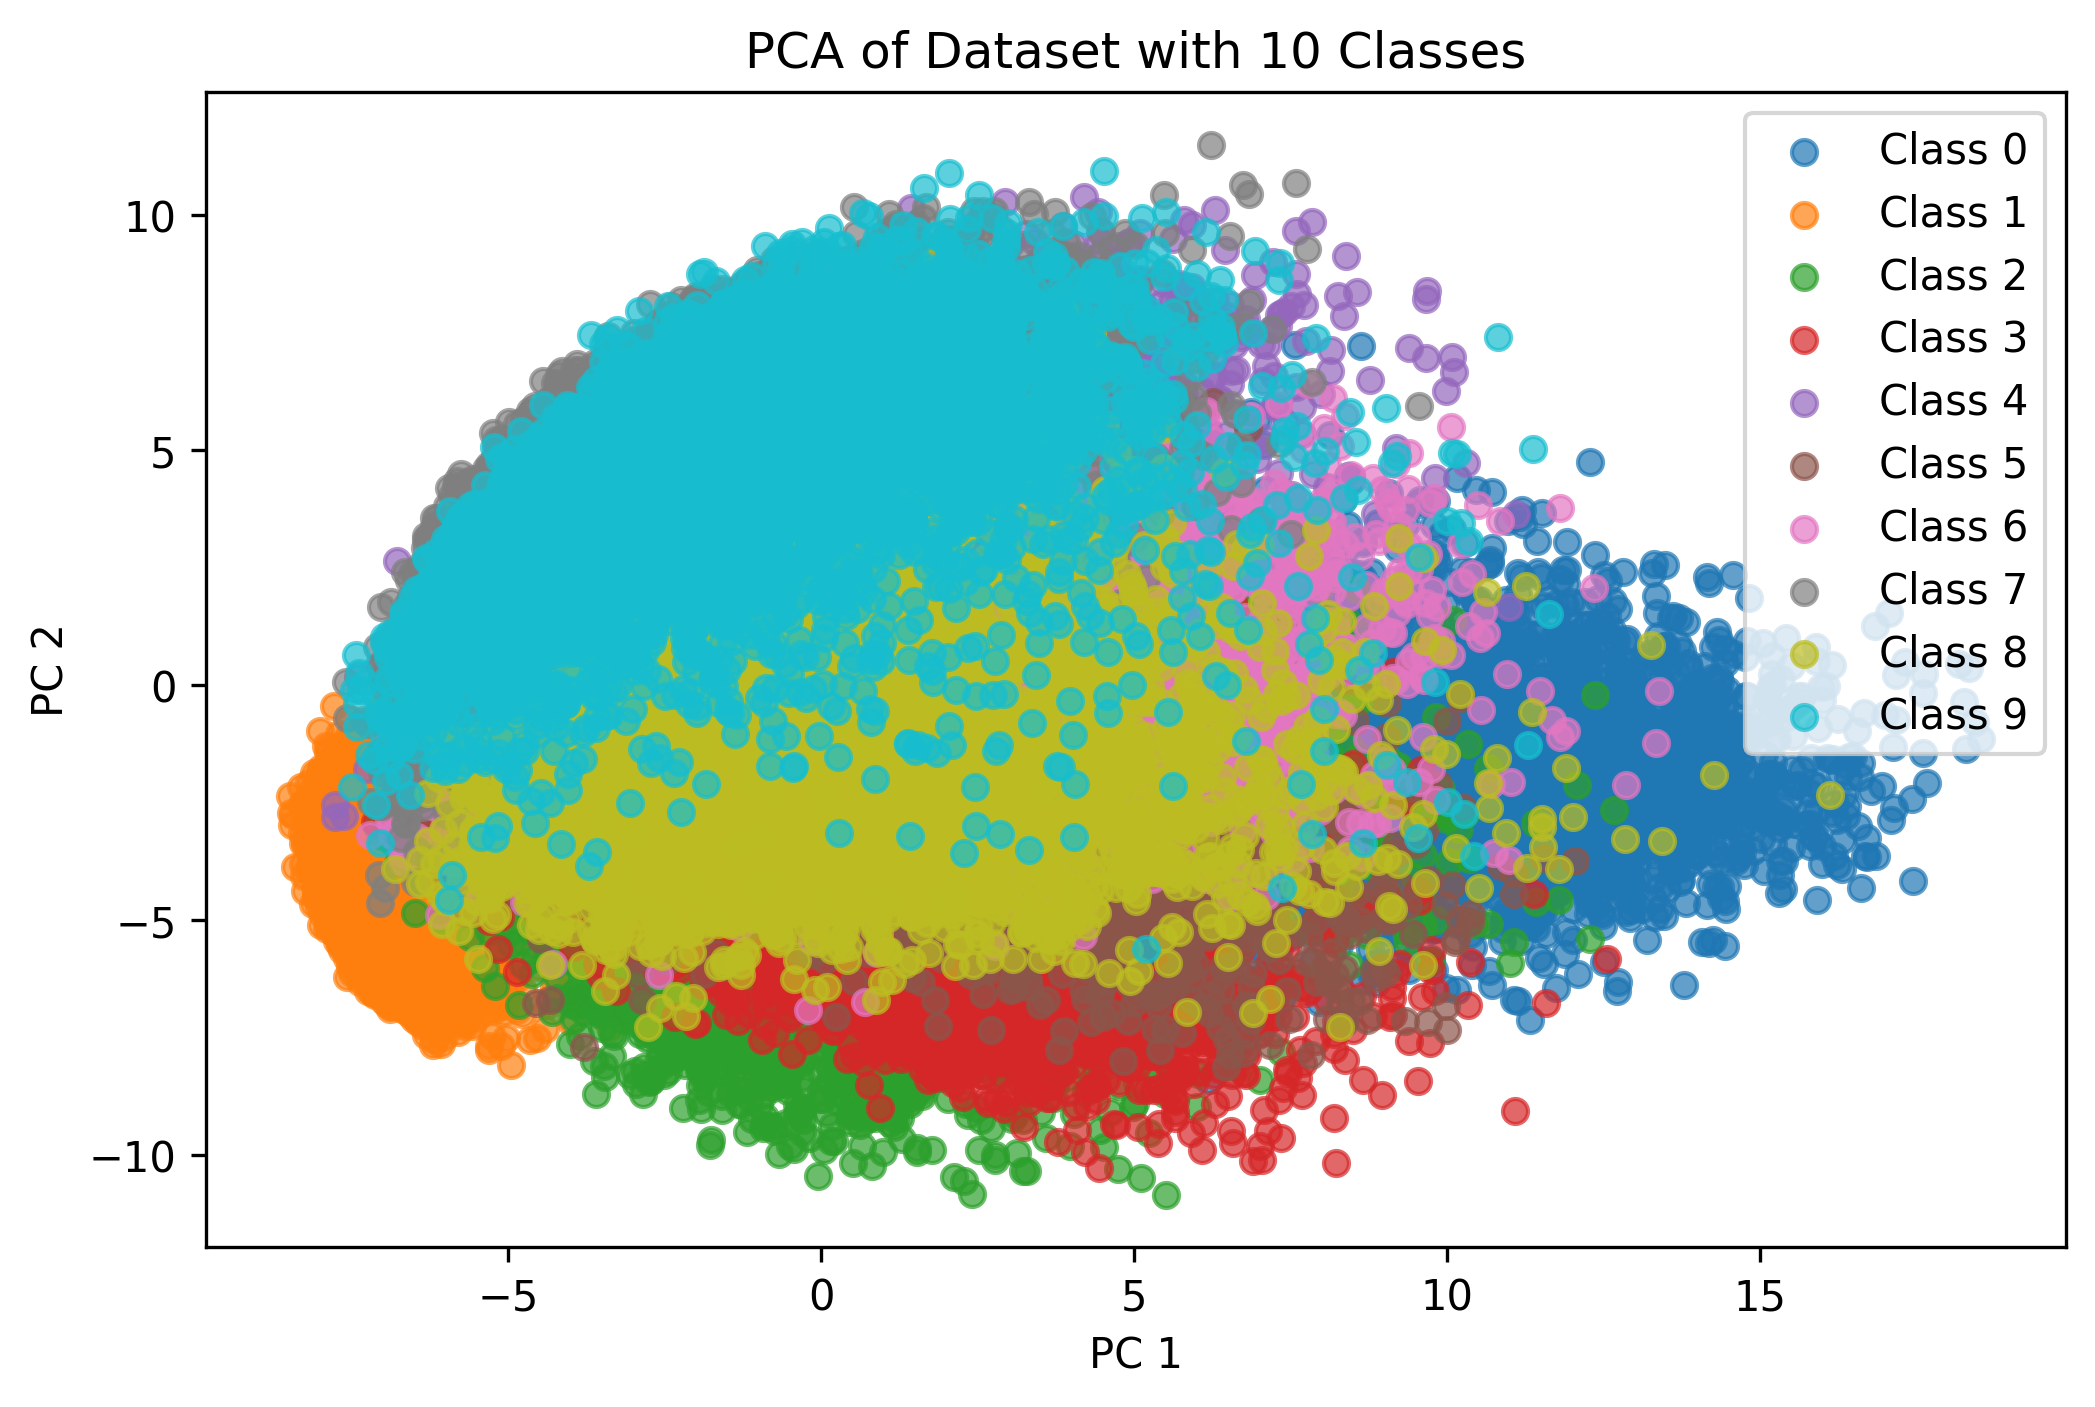
\includegraphics[width=0.5\textwidth]{./plots/plot1.png}  % Replace 'example-image' with your file name
    \caption{Plot of 2 first components of PCA for all digits of the MNIST dataset.}
    \label{fig:plot1}  % Label for referencing the figure
\end{figure}

If we plot the first two components with different colour for each class, we can see which classes overlap, and which ones are linearly separable.
Thus we have that, for example, the pairs (0, 1), (0, 2), and (2, 9) should be easy to differentiate since the occupy opposing parts on the plane.
Still, due to the significant overlap caused by 10 different classes, the distribution of some of the classes is obscured. 

\begin{figure}[h!]
    \centering
    % First subfigure
    \begin{subfigure}[t]{0.45\textwidth}
        \centering
        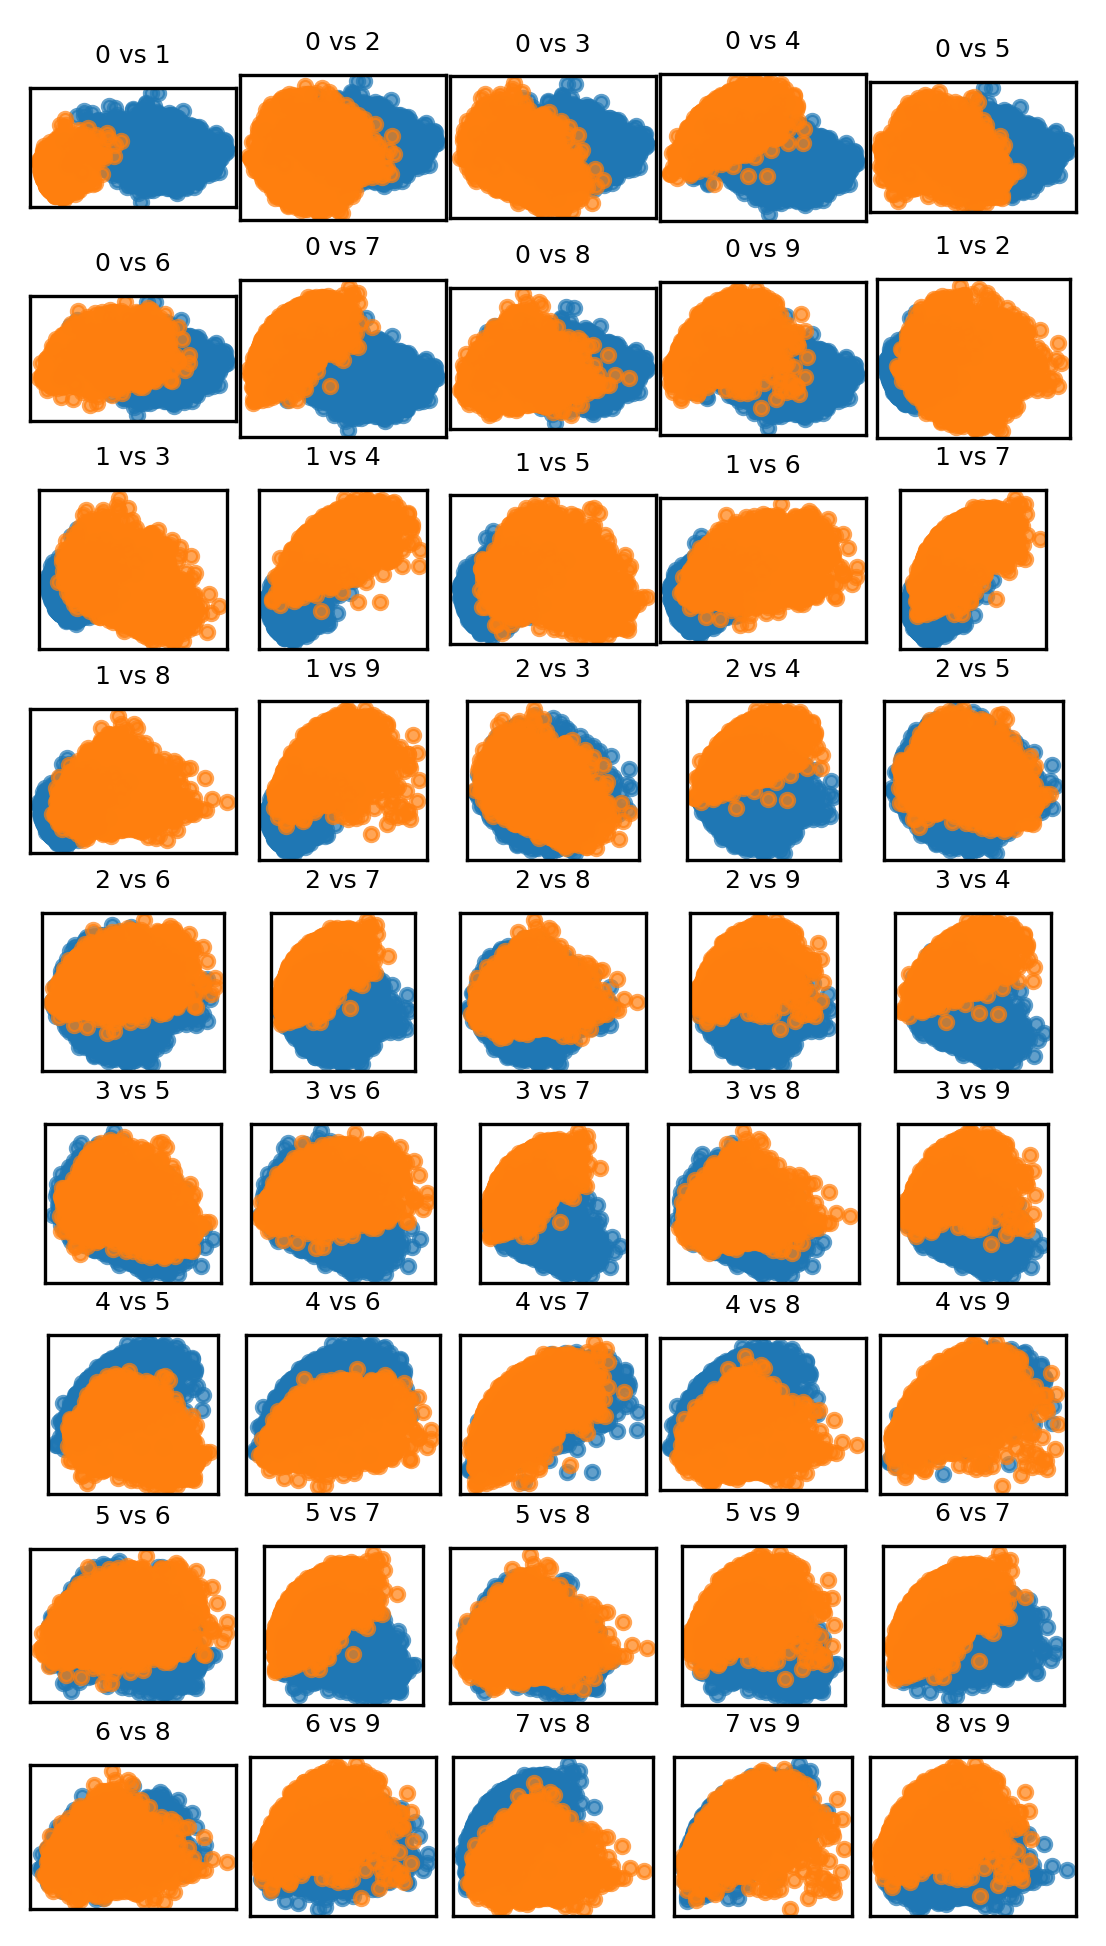
\includegraphics[width=\textwidth]{./plots/plot2.png} % Replace with your first image
        \caption{Plot of the first 2 PCA Components for all pairs of digits.}
        \label{fig:plot2a}
    \end{subfigure}
    \hspace{0.02\textwidth}
    % Second subfigure
    \begin{subfigure}[t]{0.45\textwidth}
        \centering
        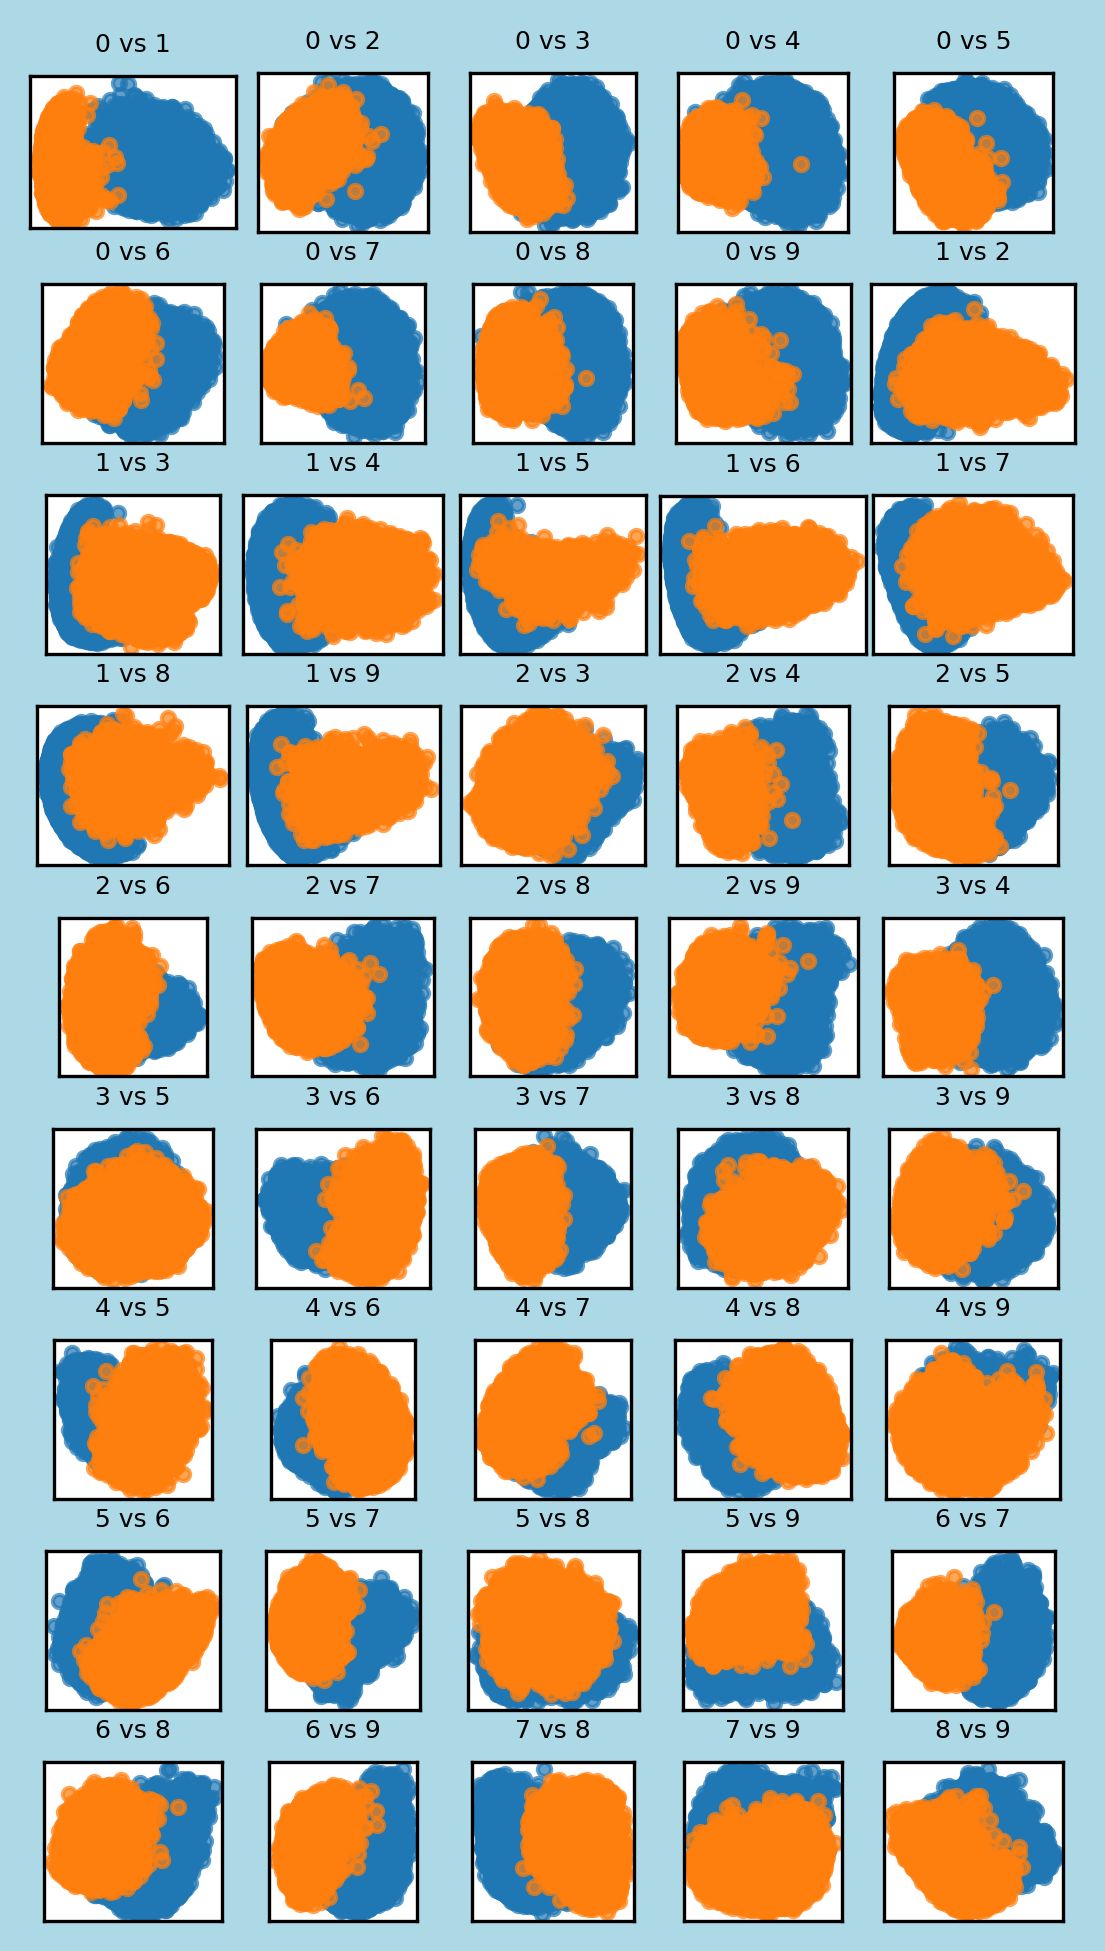
\includegraphics[width=\textwidth]{./plots/plot3.png} % Replace with your second image
        \caption{Pair-wise PCA plot.}
        \label{fig:plot2b}
    \end{subfigure}
    % Main caption for the figure
    \caption{Side-by-side visualization of PCA components and pair-wise PCA plots.}
    \label{fig:side_by_side}
\end{figure}

Figure 2a provides a pairwise visualisation of the distributions.
It Is clear that some pairs of classes, e.g. (0, 1), (0, 7), (3, 7) are relatively distinct, while others (5, 8), (7, 9) are virtually impossible to separate.
However it must be kept in mind that this is the result of considering just 2 components and not all of the information contained in the dataset.
That means distributions that do not seem differentiable now, may actually be when the model is trained on the original dataset.
What is more, the above results are obtained by performing PCA on the whole dataset.
However, when it comes to distinguishing classes in pairs, the datapoints of other classes introduce variance and noise that may be irrelevant.
Thus, it is worth producing the same plot with the PCA calculated for each pair.
This is shown in figure 2b and it becomes apparent that the results are better in terms of separability.
To objectively measure this, we use the silhouette score which takes into account the average distance of a clusters samples between each-other and between the samples of the other class.
Higher scores mean better clustering and for the generic PCA we get 0.337 where as the same score for the pairwise PCA is 0.407.
This proves that we can achieve better clustering (and hence prediction performance) by performing pairwise PCA.


\subsection{Mathematical basis of PCA}
Before applying and transformations on the dataset, it is important to normalize it so the features with larger ranges do not affect the calculations disproportionately. 

\begin{figure}[h!]
    \centering
    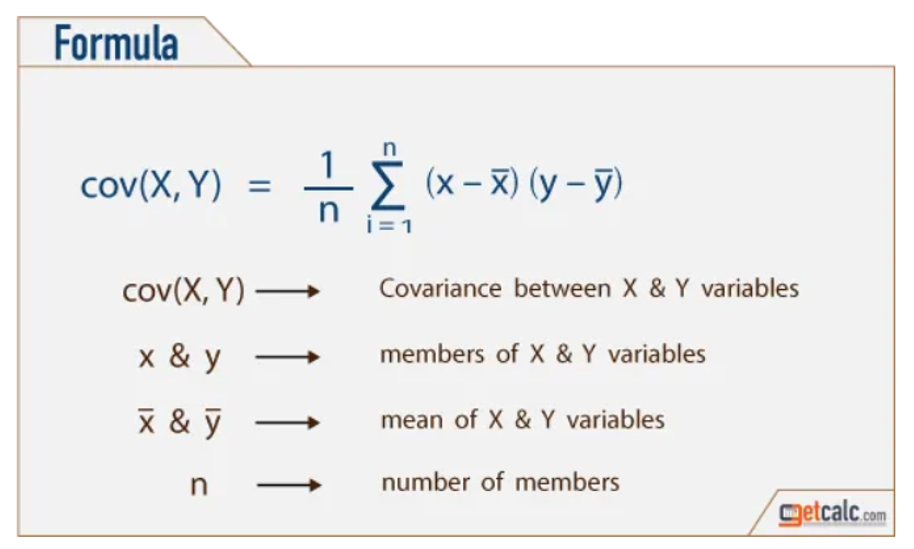
\includegraphics[width=0.5\textwidth]{./plots/plot4.png}  % Replace 'example-image' with your file name
    \caption{Calculation of Covariance Matrix (Dubey, 2018).}
    \label{fig:plot5}  % Label for referencing the figure
\end{figure}

The next step is to identify how much each feature correlates with the other ones, as the more they correlate, the less useful information they add.
Figure 4 shows the steps of calculation, which essentially shows that the more two variables follow the same trend, then larger the product of their difference to the mean will be

From Linear Algebra we know that a matrix can represent a transformation and its eigenvectors represent the directions in which the data has the most variance.
Thus these eigenvectors will form the basis of the new vector space which is now built so that each new dimensions contains the most variance

The actual amount of variance explained by each dimension is given away by the eigenvalues of the eigenvectors.
We can create a new matrix by concatenating the desired number of eigenvectors which, when multiplied with our data, produces the PCA-Data, which is our data transformed to the new base. 

\section{Perceptrons (Task 2)}

The human neurons can receive multiple stimulations that are then upregulated or downregulated by special chemicals at the neural synapses.
The result then is not a linear stimulation but instead a binary state of excitation which closely resembles what we humans would call “making a decision” (Glasgow University).
Rosenblatt’s perceptron machine  is a software analogous which receives a multidimensional input that it scales individually, and then compares its sum to a bias in order to select one of two kinds of responses (Cornell University).
In that case, the input can be the coordinates of some samples that we know belong in different classes, and that we would like the machine to be able to distinguish.
The weights and the bias are independent of the input and can be set up to do exactly that.
Since the operation of scaling with a parameter and then subtracting another is the equation of the line (in two dimensions) or a hyperplane, we can set up an algorithm that hypotheses which plane would separate these classes based on the values of their coordinates, and if this hypothesis is wrong, it changes it so that it would work well for these specific samples.
If the samples occupy distinct areas of the feature space and we do that for all samples, the resulting hyperplane  would end up satisfying the requirement for all samples (since we know the samples of a cluster have similar feature values).
From Task 2 we know that this applies to a degree, for the digit pairs.

The algorithmic approach consists of two functions.
The first implements the matrix multiplication/scaling and the comparison with the threshold to return a result/decision.
The second iterates through the samples of the dataset, producing a prediction and then correcting the weights so that if the prediction was wrong, next time it will be closer to right.
The algorithms stops upon achieving an MSE goal or reaching the iterations threshold.
With each iteration the number of misclassifications reduces on the training dataset, but the same is not always true for the test dataset, as the two contain different samples and too accurate a modeling of the training samples can end up imprinting noise on the model (overfitting).
This is demonstrated by the training vs test accuracy, over number of iterations in figure 4.

\begin{figure}[h!]
    \centering
    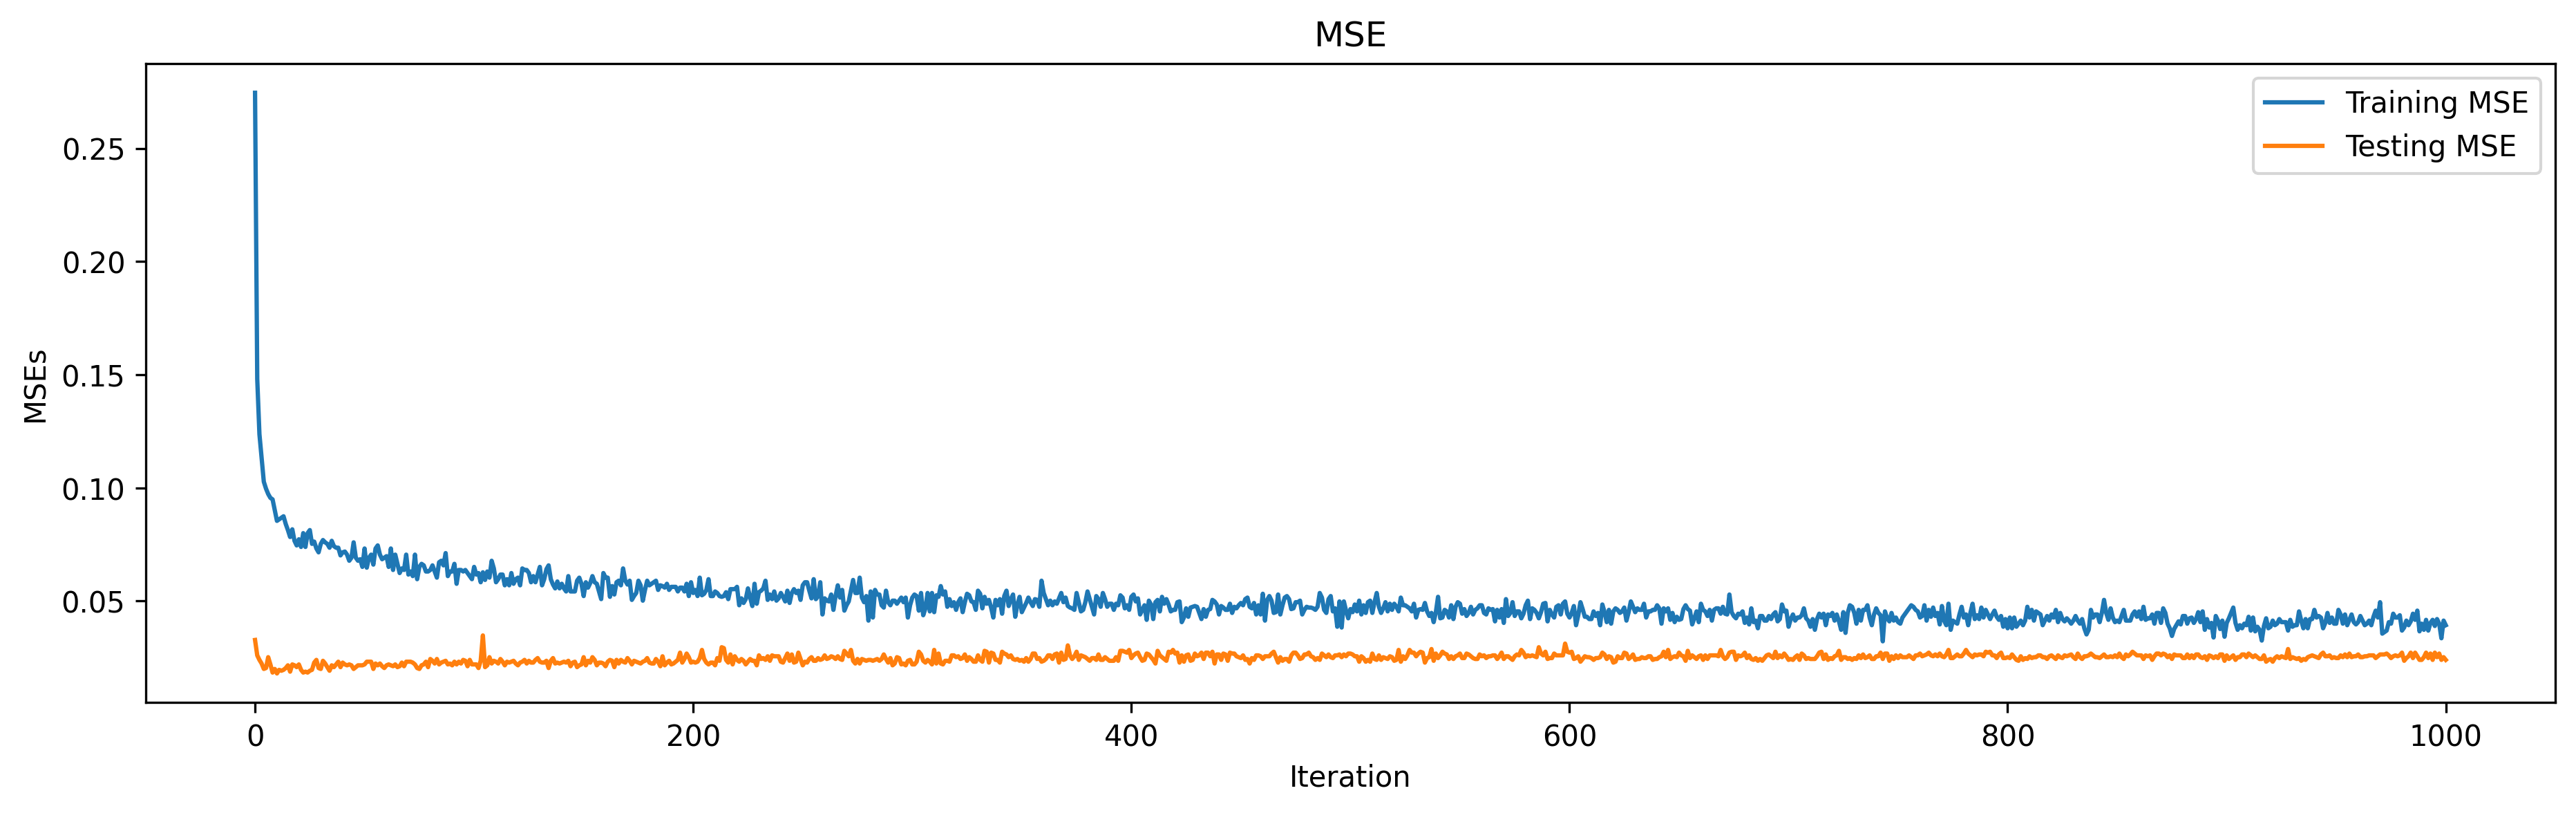
\includegraphics[width=\textwidth]{./plots/plot5.png}  % Automatically scales to page width
    \caption{Training vs Testing Mean Square Error (MSE).}
    \label{fig:plot6}  % Label for referencing the figure
\end{figure}

On one hand it is clear that peak accuracy is achieved at 10-20 iterations, after which the reduction in training MSE seems to indicate overfitting rather than actual improvement.
Since the weights are randomly initialized at each run, multiple runs equal to simulated annealing and can serve to expose entrapment to local minimum.
As the MSE is repeatedly similar, we can infer that the algorithm does not converge to a poor local minimum.

Still, given the baseline MSE calculated in the notepad as 3.6, it is evident that the model has actually learned to distinguish between the two classes (8 and 9).
The weights matrix has the same properties as the input matrix and thus, be reversing the process of transforming the digit images to input arrays, we can produce an image of the learned weights.
Figure 5a provides this visualization, and makes clear that this particular simple model does not learn any high level features a human would use.
Instead it may opportunistically utilize whichever pixels help it correctly split groups of samples that the training so far has not been able to assist it with, similar to nodes that split high impurity leaves in decision trees.
Figure 4 shows the difference between the average image of 8 and 9.
Areas with high or low brightness indicate consistent differences between the classes that could be used for a rule based system, yet we see that the model has focused elsewhere.


\begin{figure}[h!]
    \centering
    % First subfigure
    \begin{subfigure}[t]{0.3\textwidth} % Adjust width as needed
        \centering
        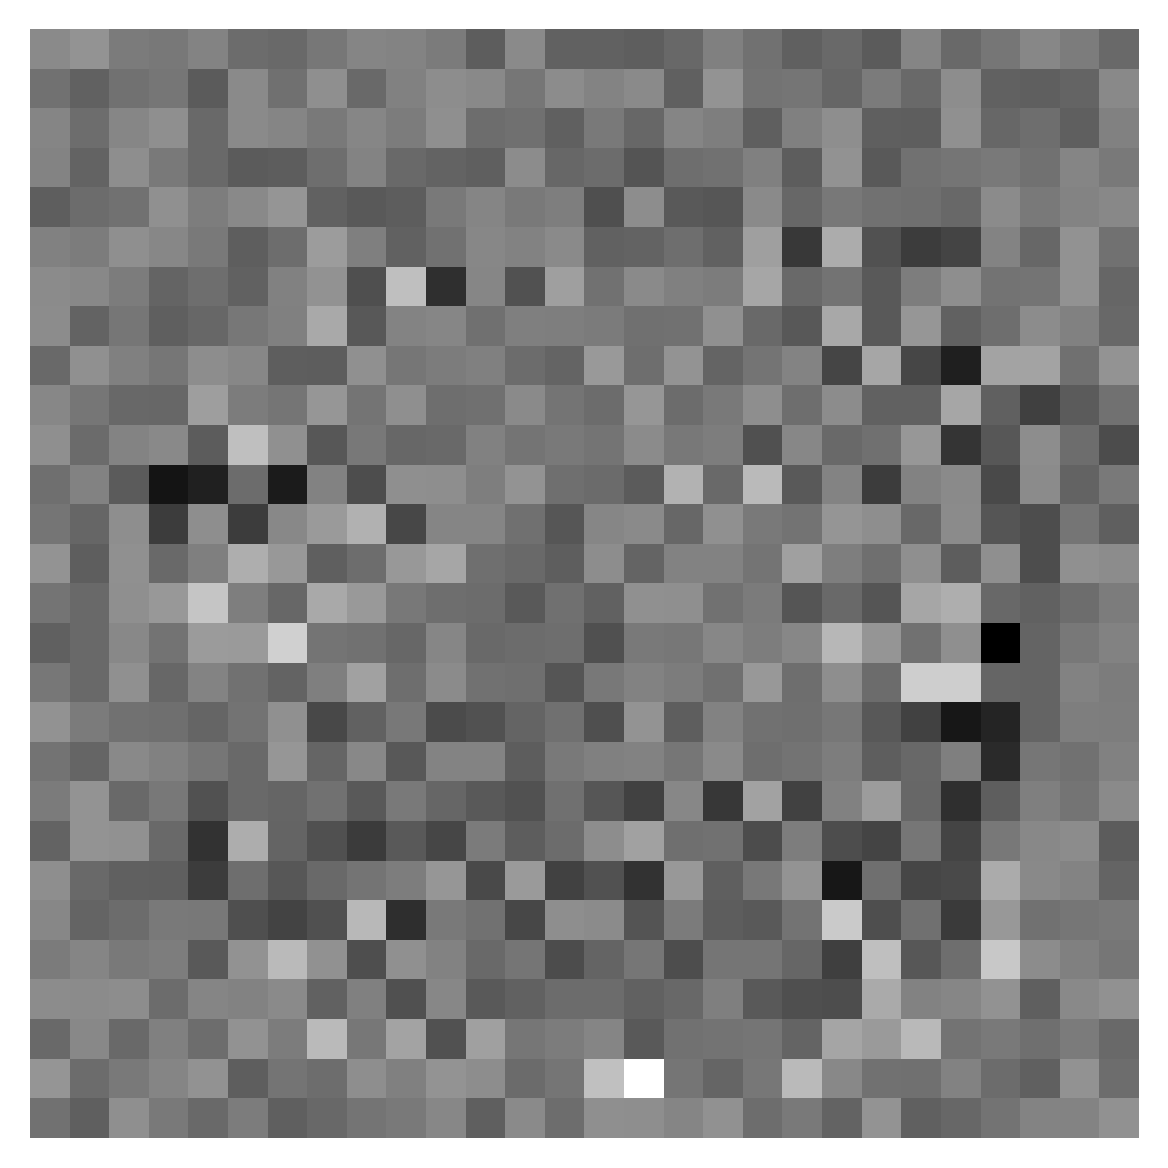
\includegraphics[width=\textwidth]{./plots/plot6.png} % Replace with your first image file
        \caption{Visualisation of weights learned by the Perceptron}
        \label{fig:plot7a}
    \end{subfigure}
    \hspace{0.01\textwidth}
    % Second subfigure
    \begin{subfigure}[t]{0.3\textwidth}
        \centering
        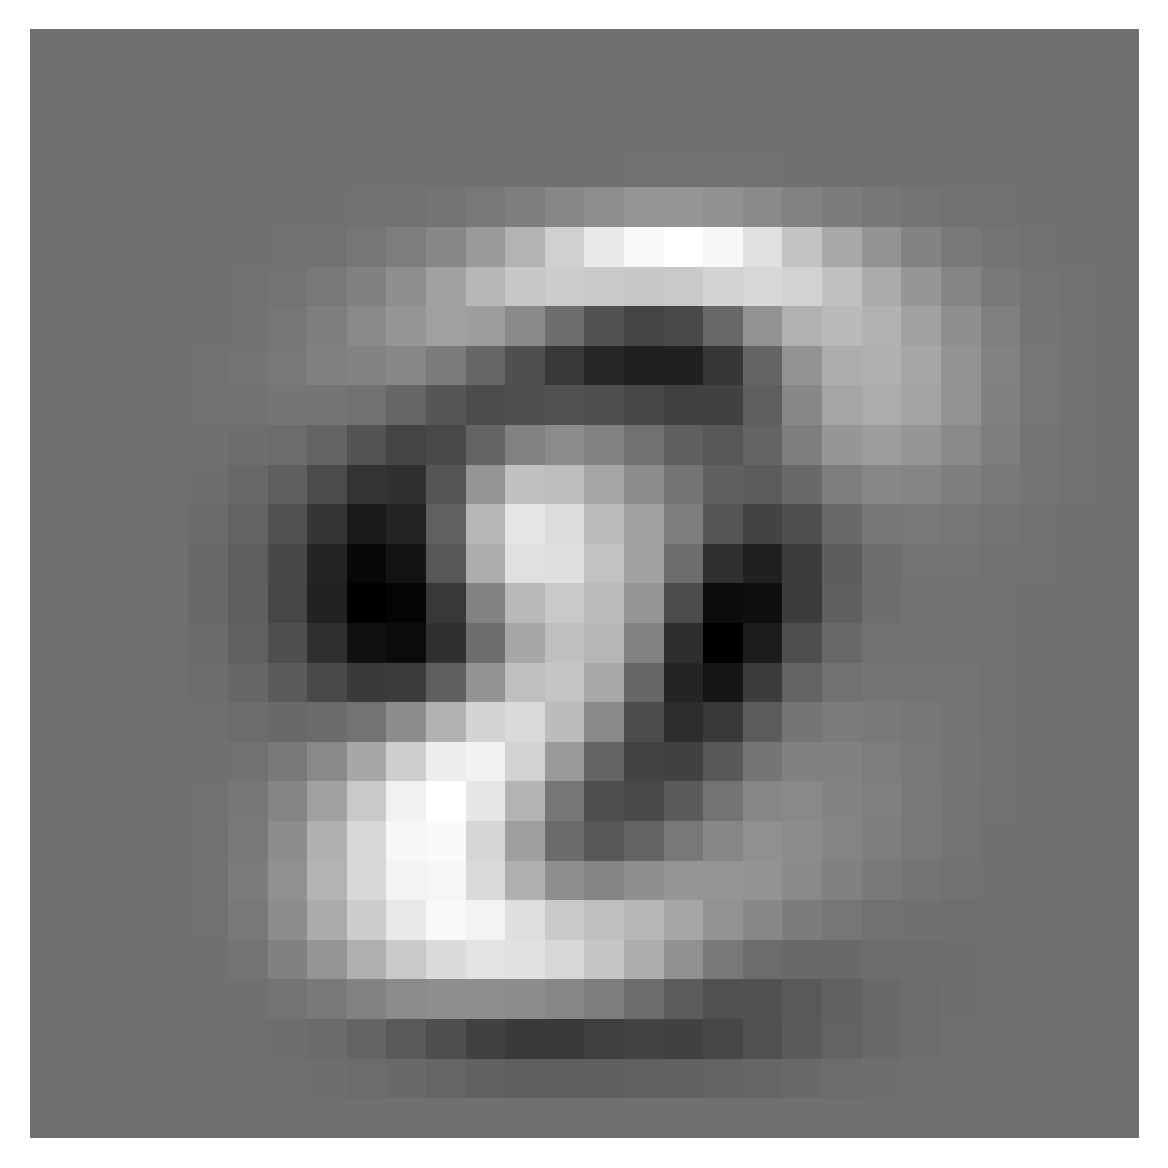
\includegraphics[width=\textwidth]{./plots/plot7.png} % Replace with your second image file
        \caption{Difference betweeen average hand-drawn 8 and 9 characters}
        \label{fig:plot7b}
    \end{subfigure}
    \hspace{0.01\textwidth}
    \begin{subfigure}[t]{0.3\textwidth}
        \centering
        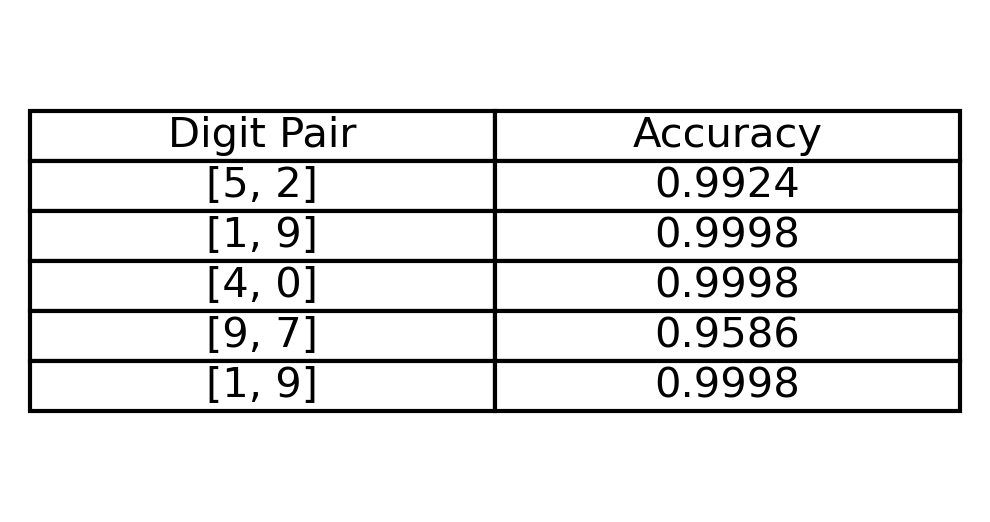
\includegraphics[width=\textwidth]{./plots/plot8.png} % Replace with your third image file
        \caption{Accuracies for various digit pairs}
        \label{fig:plot7c}
    \end{subfigure}

    % Main caption for the entire figure
    \caption{Main caption describing all three subfigures.}
    \label{fig:main_figure}
\end{figure}

Figure 6 is a compilation of other pairs of digits with the respective achieved accuracy after training.
We see variations that are aligned with how visually similar the two digits are.
It must be kept in mind that handwritten digits have different shapes that the digitally displayed ones, for example, the digit ‘5’ is often drawn as an ‘S’, which is more easily interpreted as an ‘8’.

\section{Multilayer Perceptrons (Task 3)}

To solve the problem of the perceptron’s simplicity, we can organize large groups of them into Neural Networks (NN).
The motivation stems from a property called “emergence” that we observe when multiple biological neurons work together, where the resulting structure achieves capabilities that exceed the sum of its parts (Pedder, 2023).
In the software domain, the model can learn complex curves to separate the classes more effectively than hyperplanes can (Choi, 2020).
Using the Keras Library we can initialize and train a network as per the assignment brief’s requirements.
Even with the architecture fixed there are various hyperparameters that define how the model works.
Number of epochs is similar to the iterations in task 2, and batch size allows the model to work with groups of samples speeding up training.
The amount of time needed to find the best combination increases exponentially with the number of parameters so using guidelines (Bengio, 2012) and some tests, we find one that is sufficient.
The resulting training and test accuracy is as follows:.

\begin{figure}[h!]
    \centering
    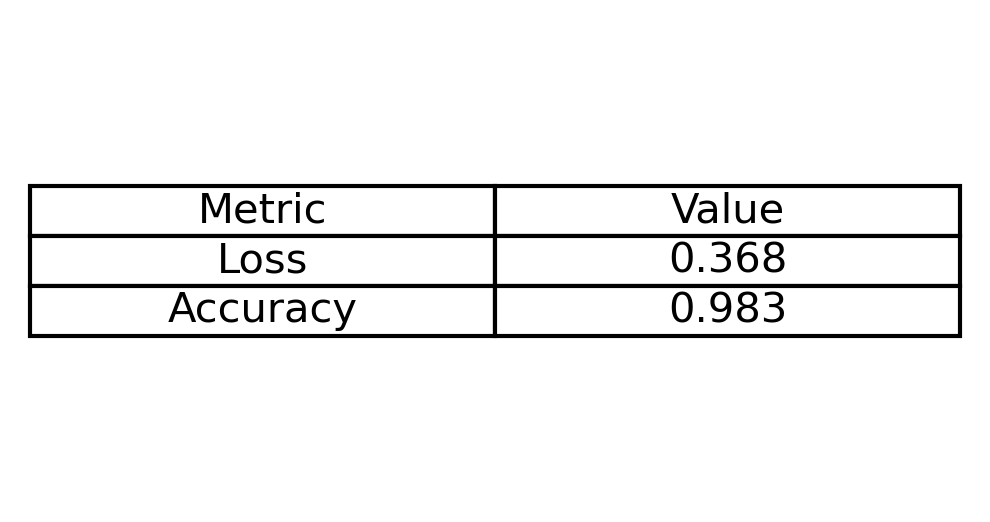
\includegraphics[width=0.3\textwidth]{./plots/plot10.png}  % Automatically scales to page width
    \caption{MLP performance metrics (on entire dataset)}
    \label{fig:plot8}  % Label for referencing the figure
\end{figure}

At first sight it might seem as if the accuracy is lower that with the perceptron.
The reason why this comparison would be misguided is that the model now performs multiclass classification, not binary classification, which is significantly more demanding.


\subsection{Math of PCA}
\subsubsection{Details}

\end{document}
